%\part{Removendo o intermediário}
\chapter{Removendo o intermediário}
\label{ch:capitulo2}

No capítulo anterior, comentamos que o Bitcoin fornece um sistema ponto a ponto para a transferência de valor. Antes de nos aprofundarmos em como isso funciona, vamos primeiro entender como um banco tradicional ou empresa de pagamento lida com o rastreamento da propriedade e das transferências de ativos.

\section*{Os bancos são apenas livros contábeis}
%\paragraph{}

Como funciona um pagamento digital feito por seu banco, PayPal ou ApplePay? Muito simples, essas entidades intermediárias atuam como um livro-razão de contas e transferências glorificado.

O proposito de um banco é armazenar seus depósitos e guardar-los. Porem depósitos hoje em dia são primariamente eletrônicos em vez de papeis ou moedas.
Então o trabalho de um banco é manter e guardar esse banco de dados bancários.
visto que a informação é eletrônica, os seguranças são majoritariamente eletrônicos.
Bancos utilizam softwares que detectam intrusos, fazem backups contra perda de informação e fazem auditorias com terceiros para ter certeza que seus processos internos não estão comprometidos, além de seguros para se protegerem caso algo de errado nesse processo.
%paragrafo adicionado

Neste exemplo, vamos utilizar a expressão \textit{banco}, mas queremos dizer realmente qualquer outra entidade que processa pagamentos. Começamos com um livro-razão de contas que mostra que Ana e Bruno depositaram dinheiro no banco.

\begin{figure}
  \centering
  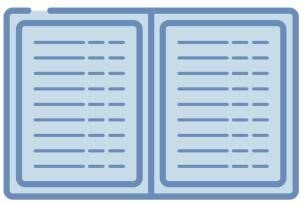
\includegraphics[width=4cm]{imagens/livro-capitulo-02.jpg}  
  \caption*{\textit{\small Livro-razão}}
\end{figure}

\paragraph{}
\textbf{Livro razão do banco}

\begin{samepage}
\begin{enumerate}
\item Ana: Crédito por depósito em dinheiro $+R\$2,00$ 
\item Bruno: Crédito por depósito em dinheiro $+R\$10,00$
\end{enumerate}
\end{samepage}

Quando Ana deseja enviar $R\$2,00$ para Bruno, ela liga para seu banco ou usa o \textit{internet banking} ou um aplicativo disponibilizado pela empresa, autentica-se usando um nome de usuário e senha ou um código PIN e, em seguida, faz a solicitação de transferência. O banco, então, registra em seu livro-razão.

\paragraph{}
\textbf{Livro razão do banco}

\begin{samepage}
\begin{enumerate}
\item Ana: Crédito para depósito em dinheiro $+R\$2,00$
\item Bruno: Crédito para depósito em dinheiro $+R\$10,00$
\item Ana: Débito $-R\$2,00$
\item Bruno: Crédito $+R\$2,00$
\end{enumerate}
\end{samepage}

Portanto, o banco registrou os novos débitos e créditos e agora o dinheiro foi movido de uma conta para outra. Simples!
%\newpage
\begin{figure}
  \centering
  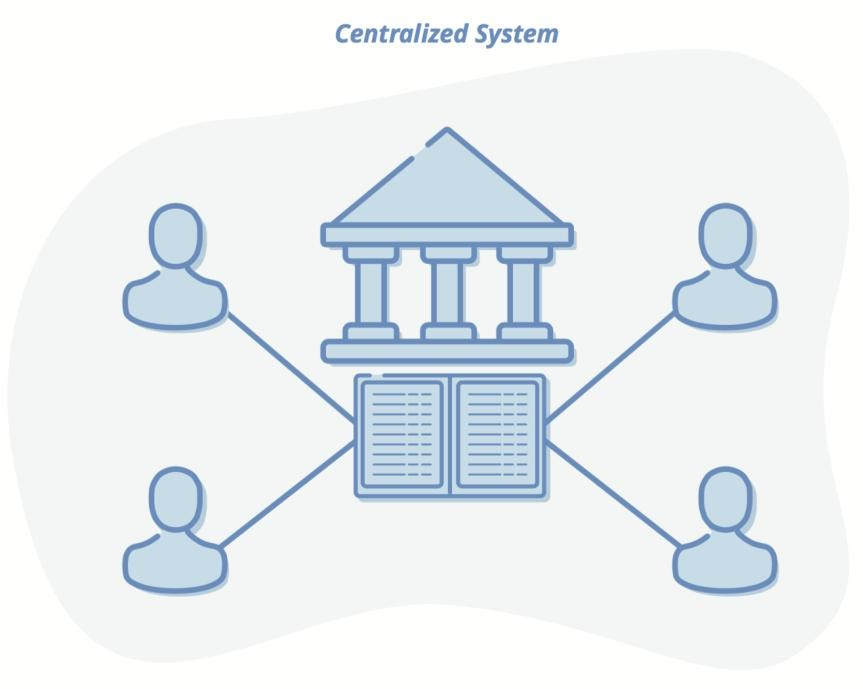
\includegraphics[width=7cm]{imagens/centralizado-capitulo-02.jpg}
  \caption*{\textit{\small Sistema centralizado}}
\end{figure}


\section*{O problema de gasto duplo}


O que acontecerá se Ana tentar gastar esses dois dólares novamente? Isso é chamado de problema de gasto duplo. Ela envia a solicitação para o banco, mas o banco diz “Desculpe, vemos que você já gastou R\$2,00 para pagar Bruno, você não tem mais dinheiro para enviar”.

Quando você tem uma autoridade central como um banco, é muito fácil para ele dizer que você está tentando gastar um dinheiro que já gastou. Isso porque eles são os únicos que podem modificar o livro-razão e têm processos internos, incluindo sistemas de backup e auditorias feitas por computadores e seres humanos para se certificar de que está correto e nada foi adulterado.

Chamamos isso de \textit{sistema centralizado} porque possui um único ponto de controle.

\paragraph{Vamos descentralizar o livro razão}
\paragraph{}

O primeiro problema que o Bitcoin visa resolver é a remoção de um intermediário confiável criando um sistema \textit{ponto a ponto}. Vamos imaginar que os bancos desapareceram e precisamos recriar nosso sistema financeiro. Mas desta vez, não vamos ter um ente central. Como podemos manter um livro-razão sem nenhum centralizador?

Se não temos um guardião do livro-razão, precisaremos que o livro-razão pertença ao povo. \textit{Vive la révolution}. É assim que fazemos.

Primeiro, vários nos reunimos e criamos uma \textit{rede}. Isso apenas significa que temos um jeito de conversar uns com os outros. Digamos que trocamos números de telefone ou contas de Snapchat. Quando Ana quiser enviar dinheiro para Bruno, ao invés de ligar para o banco, ela vai no Snapchat de todos os seus amigos e diz a eles: “Estou enviando R\$2,00 para Bruno”. Todos a reconhecem, respondendo "Legal, entendemos!", e escrevem em suas cópias do livro-razão. A imagem agora tem a seguinte aparência:

~

\begin{figure}
  \centering
  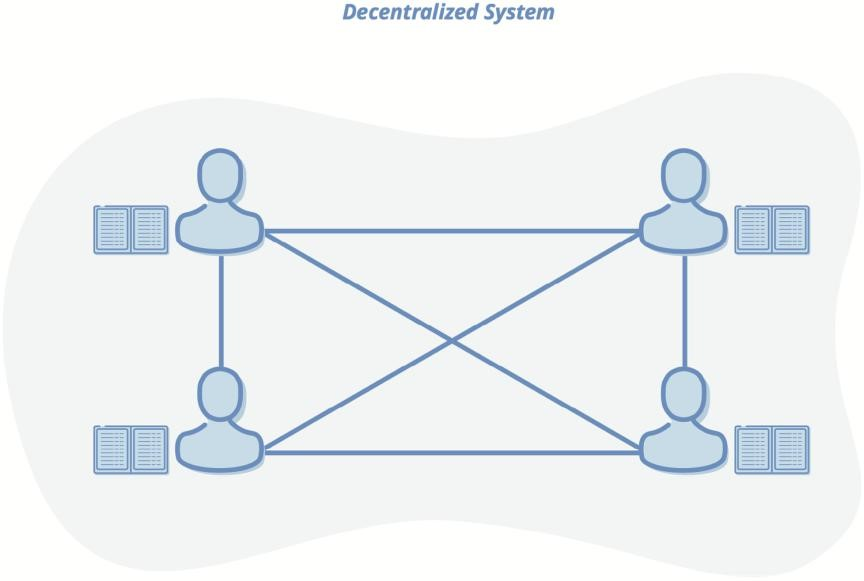
\includegraphics[width=10cm]{imagens/descentralizado-capitulo-02.jpg}
  \caption*{\textit{\small Sistema descentralizado}}
\end{figure}
%\newpage

Portanto, ao invés de um único banco, temos uma cópia do livro-razão nas mãos de todos. Sempre que alguém quer gastar o dinheiro, basta ligar ou fazer um snapchat a todos os seus amigos e informá-los de que isso está acontecendo. Todos registrarão as transações. Como o livro-razão não está mais em apenas um lugar, nós o chamamos de \textit{distribuído} e, como nenhum ente centralizado é responsável, o chamamos de \textit{descentralizado}.
Isso resolve o problema do intermediário confiável

Agora que não temos intermediário, como isso resolve o problema do gasto duplo? Quem devemos consultar invés do banco para verificar se dinheiro já foi gasto ou não? Bem, uma vez que todos possuem uma cópia do livro-razão, todos devem ser consultados. Esse sistema é conhecido como sistema baseado com consentimento porque ele precisa que todos concordem com uma versão particular da verdade.%paragrafo adicionado

se Ana tentar gastar novamente os R\$2,00 que ela já enviou para Bruno, sua transação será rejeitada por todos na rede, já que eles consultariam seus livros-razão e diriam a ela que de acordo com seus registros, ela já gastou o dinheiro.
Portanto, eles não iriam registrar sua segunda tentativa de gastar o dinheiro. Agora temos uma rede ponto a ponto para registrar propriedade e transferências de fundos.

Este sistema funciona muito bem entre um grupo de amigos que têm motivos sociais para não enganar uns aos outros, mas isso não se aplica quando as redes possuem milhões de pessoas. 
À medida que mais e mais pessoas começam a usar o sistema, há um incentivo para trapacear para obter dinheiro extra no livro-razão.

Como mantemos todos honestos?

\section*{O ataque de gastos duplos}
%\paragraph{}

Se eu for a Ana, posso \textit{conspirar} com algumas das outras pessoas e dizer a elas: "Quando eu gastar o meu dinheiro, não escreva em seus livros. Finja que essa transação nunca aconteceu”. Veja como Ana pode realizar um ataque de gasto duplo.

Começando com um saldo de $R\$2,00$, Ana faz o seguinte:

\begin{enumerate}
\item Ela manda seus $R\$2,00$ para Bruno, para comprar uma barra de chocolate. Agora ela deve ter $R\$0,00$ sobrando;
\item Danilo, Evandro e Fernanda estão conspirando com Ana e não registram a sua transação para Bruno em seus livros. Em sua cópia, Ana nunca gastou seu dinheiro;
\item Carol é uma honesta guardiã do livro-razão. Ela anota a transação de Ana para Bruno. Em seu livro-razão, Ana tem $R\$0,00$;
\item Henrique estava de férias por uma semana e não ouviu falar de nenhuma dessas transações. Ele se junta à rede e pede uma cópia do livro-razão;
\item Henrique obtém 4 cópias falsas (Danilo, Evandro, Fernanda, Ana) e uma cópia honesta (Carol). Como ele determina qual é a real? Sem um sistema melhor, ele busca a maioria dos votos e é enganado ao aceitar o livro-razão falso como sendo o correto;
\item Ana compra uma barra de chocolate de Henrique usando os $R\$2,00$ que ela realmente não tem. Henrique aceita porque, pelo que sabe, Ana ainda tem $R\$2,00$ em sua conta (de acordo com o livro-razão que ele obteve de todos os outros;
\item Ana agora tem 2 barras de chocolate e $R\$4,00$ de dinheiro falso foram criados no sistema. Ela paga seus amigos em barras de chocolate, e eles repetem o ataque 100 vezes a cada nova pessoa que entra na rede;
\item Agora, Ana tem todas as barras de chocolate e todos os outros estão segurando grandes quantias de dinheiro falso;
\item Quando eles tentam gastar o dinheiro que Ana supostamente enviou para eles, Danilo, Evandro e Fernanda que controlam a maioria da rede, rejeitam esses gastos porque sabem que o dinheiro é falso desde o começo.
\end{enumerate}

Nós temos um problema. Isso é chamado de \textit{falha de consenso}. As pessoas na rede não chegaram a um consenso sobre qual é o estado real. Não tendo um sistema melhor, eles seguiram a regra da maioria, o que levou a pessoas desonestas controlando a rede e gastando dinheiro que não tinham.

Se quisermos fazer um sistema \textit{sem permissão} onde qualquer um pode participar sem pedir, então ele também deve ser resiliente a usuários desonestos.

\section*{Resolvendo o problema de consenso distribuído}
%\paragraph{}
Agora vamos resolver um dos problemas mais difíceis da ciência da computação: consenso distribuído entre as partes, onde alguns são desonestos ou não confiáveis. Este problema é conhecido como Problema dos Generais Bizantinos e é a chave que Satoshi Nakamoto usou para criar a invenção do Bitcoin. Vamos começar de forma simples.

Precisamos fazer com que várias pessoas concordem com os dados do livro-razão sem saber se os  responsáveis pelo livro-razão têm anotado todas as transações de maneira correta e honesta.

Uma solução ingênua é simplesmente nomear os representantes honestos do livro-razão. Em vez de todos começarem a escrever nele, escolhemos um punhado de amigos como Carol, Giovana, Fernanda e Zélia para fazer isso, porque eles não mentem e todo mundo sabe que nunca vão para as festas nos fins de semana.

Então, toda vez que temos que fazer uma transação, em vez de contar a todos os nossos amigos, apenas ligamos para Carol e a sua gangue. Eles ficam felizes em manter o livro-razão para nós por uma pequena taxa. Depois de escreverem no livro-razão, eles ligam para todos os outros e informam sobre as novas linhas incluídas, que todos ainda mantêm como backup.

Este sistema funciona muito bem, exceto que um dia, agentes do governo aparecem e querem saber quem está administrando este sistema financeiro paralelo. Eles prendem a Carol e seus amigos e os levam embora, pondo fim ao livro-razão distribuído. Todos nós temos backups não confiáveis, não podemos confiar uns nos outros e não podemos descobrir de quem é o backup que deve ser usado para iniciar um novo sistema.

Em vez de um fechamento total, o governo também pode ameaçar discretamente os responsáveis pelo registro com pena de prisão se eles aceitarem as transações da Ana (que é suspeita de vender drogas). O sistema agora está efetivamente sob controle central e não podemos mais dizer que ele não tem permissão.

E se tentarmos a democracia? Vamos encontrar um grupo de 50 pessoas honestas e realizaremos eleições todos os dias para manter a rotação de quem escreve no livro-razão. Todos na rede têm direito a voto.

Este sistema funciona muito bem até que as pessoas apareçam e usem violência ou coerção financeira para alcançar os mesmos objetivos de antes:

\begin{samepage}
\begin{enumerate}
\item Forçar o eleitorado a votar nos contadores de sua escolha;
\item Forçar os detentores do livro-razão eleitos a escreverem lançamentos falsos nele.
\end{enumerate}
\end{samepage}

Nós temos um problema. Sempre que designamos pessoas específicas para manter o livro-razão, devemos confiar que elas são honestas, e não temos como defendê-las de serem coagidas por alguém a cometer atos desonestos e corromper nosso livro-razão.

\section*{Identidade equivocada e ataques Sybil}
%\paragraph{}
Até agora, examinamos dois métodos fracassados de garantir a honestidade: um usava contadores específicos e conhecidos e o outro usava contadores eleitos e rotativos. A falha de ambos os sistemas foi que a base de nossa confiança estava ligada à identidade do mundo real: ainda tínhamos que identificar especificamente os indivíduos que seriam responsáveis por nosso livro-razão.

Sempre que assumimos confiança com base na identidade, nos abrimos para algo chamado \textit{Ataque Sybil}. Este é basicamente um nome chique para personificação; tem o nome de uma mulher com transtorno de personalidade múltipla.

Você já recebeu uma mensagem estranha de um de seus amigos apenas para descobrir que o telefone dele havia sido pego pelo irmão? Quando se trata de bilhões ou mesmo trilhões de dólares em jogo, as pessoas justificam todo tipo de violência para roubar aquele telefone e enviar aquela mensagem. É fundamental evitarmos que as pessoas que mantêm nosso livro-razão sejam coagidas de alguma forma. Como podemos fazer isso?

\section*{Vamos construir uma loteria}
%\paragraph{}
Se não queremos a possibilidade de pessoas serem comprometidas por ameaças de violência ou suborno, precisamos de um sistema com tantos participantes que seria impraticável para alguém coagi-los. Deve ser o caso de que qualquer pessoa possa participar de nosso sistema, e que não tenhamos que introduzir nenhum tipo de votação, que está sujeita à coerção pela violência e compra de votos.

E se fizéssemos uma loteria onde escolheríamos alguém aleatoriamente sempre que quiséssemos escrever no livro-razão? Aqui está nosso primeiro rascunho deste design:

\begin{samepage}
\begin{enumerate}
\item Qualquer pessoa no mundo pode participar. Dezenas de milhares de pessoas podem aderir à nossa rede de loteria de contadores;
\item Quando queremos enviar dinheiro, anunciamos para toda a rede as transações que pretendemos realizar, tal como o fizemos anteriormente;
%na minha versao ta assim:
\item Invés de todas as pessoas anotarem a transação, fazemos uma loteria para ver quem ganha o direito de adicionar as transações no livro razão.
%\item A cada dez minutos, selecionaremos um vencedor (Como? Ainda não tenho certeza); 
\item Quando selecionamos um vencedor, essa pessoa escreve todas as transações sobre as quais acabou de ouvir no livro razão;
\item Se a pessoa gravar transações válidas (conforme considerado por todos os outros participantes da rede) no livro-razão, ela receberá uma taxa;
\item Todos mantêm uma cópia do livro-razão, adicionando as informações que o último ganhador da loteria produziu;
\item Usamos o intervalo de dez minutos para garantir que a maioria das pessoas tenha tempo para atualizar seus livros contábeis entre os sorteios da loteria.
\end{enumerate}
\end{samepage}

Este sistema é uma melhoria. É impraticável comprometer os participantes deste sistema porque é impossível saber quem são os participantes e qual será o próximo vencedor.

Porem, não temos uma clara resposta para como administrar uma loteria sem alguém no comando, ou por que deveríamos confiar que o vencedor da loteria irá agir honestamente quando for escrever no livro-razão. Vamos descobrir como solucionar isso a seguir.

